\documentclass[conference]{IEEEtran}
\usepackage{booktabs,graphicx,amsmath,amssymb,cite,url,array,xcolor,tikz}
\usetikzlibrary{arrows.meta,positioning,fit}
\usepackage[T1]{fontenc}
\graphicspath{{figures/}}
% include generated fragments; show a visible TODO if one is missing
\newcommand{\safeinput}[1]{\IfFileExists{generated/#1.tex}{\input{generated/#1.tex}}{\textbf{\color{red}[TODO: generated/#1.tex missing -- run src/report\_assets.py]}}}
\newcommand{\safefig}[3]{\IfFileExists{figures/#1.pdf}{\includegraphics[width=#2]{#1}}{\textbf{\color{red}[TODO: figure #1 missing]}}}
\newcommand{\safepng}[2]{\IfFileExists{figures/#1.png}{\includegraphics[width=#2]{figures/#1.png}}{\textbf{\color{red}[TODO: add screenshot figures/\detokenize{#1}.png]}}}
\newcommand{\todo}[1]{\textbf{\color{red}[TODO: #1]}}
\newcommand{\sm}{\small}
\begin{document}
\title{Fine-Tuning a Small Decoder for Clinical-Trial Criterion Eligibility, with a From-Scratch KV Cache, Tiled Attention and Speculative Decoding}
\author{\IEEEauthorblockN{Seerat E Zahra (23i-0640)}
\IEEEauthorblockA{FAST-NUCES Islamabad, Generative AI -- Assignment 2\\
Code: \url{https://github.com/Seeratzahra500/GenAI-Assignment2}}}
\maketitle

\begin{abstract}
We fine-tune Qwen2.5-1.5B-Instruct with LoRA on the expert annotations of TrialGPT-Criterion-Annotations to predict, for a patient note and one trial criterion, an eligibility label and the supporting sentence IDs. Using a patient-grouped 37/8/8 split we compare the base and fine-tuned models with criterion-level metrics, and analyse errors. We also implement, and benchmark against references, a KV-cache decoder, a tiled online-softmax attention kernel, and greedy speculative decoding with a LoRA-tuned Qwen2.5-0.5B draft, and expose everything in a Gradio app. Fine-tuning raises test accuracy from 0.107 to 0.748 and evidence micro-F1 from 0.182 to 0.536. Rare classes remain weak, and speculative decoding was slower than cached greedy decoding in our setting; we report both honestly. The prototype is educational and not a clinical decision tool.
\end{abstract}

\begin{IEEEkeywords}
LoRA, clinical trial matching, KV cache, online softmax, speculative decoding
\end{IEEEkeywords}

\section{Introduction}
Matching patients to clinical trials requires judging each inclusion and exclusion criterion against a free-text note. TrialGPT \cite{trialgpt} showed that LLMs can do this and released expert criterion-level annotations. We study whether a small open-weight decoder, adapted with LoRA \cite{lora} on a single 16~GB GPU, can learn the task, and we implement the decoding machinery (KV cache, tiled attention \cite{flash,milakov}, speculative decoding \cite{leviathan,chen}) ourselves so that every component can be verified against a reference.

\section{Related Work}
\textbf{Clinical trial matching.} TrialGPT \cite{trialgpt} decomposes matching into criterion-level eligibility labels with evidence sentences and uses GPT-4 prompting; its expert annotations are the benchmark used here, while its GPT-4 outputs are never used as input or for evaluation. Prompting a large proprietary model is accurate but not locally executable, so we instead adapt a small open-weight decoder.
\textbf{Parameter-efficient adaptation.} LoRA \cite{lora} freezes the base weights and trains low-rank updates, which fits a 1.5B model on one 16~GB GPU; QLoRA \cite{qlora} additionally quantises the base weights, which we did not need at this scale.
\textbf{Efficient attention.} Standard attention materialises a $T\times T$ score matrix. Online softmax \cite{milakov} and its blocked use in memory-efficient attention \cite{rabe} and FlashAttention \cite{flash} compute exact attention with $O(T)$ extra memory; FlashAttention fuses this into one GPU kernel. Our PyTorch version reproduces the algorithm for verification, not for speed.
\textbf{Inference.} Caching keys and values removes the quadratic recomputation during generation \cite{pope}; grouped-query attention \cite{gqa} shrinks the cache (Qwen2.5-1.5B has 2 KV heads for 12 query heads), and rotary position embeddings \cite{rope} make explicit position handling necessary when a cache is reused. Speculative decoding \cite{leviathan,chen} lets a small draft model propose tokens that the target verifies in one pass, giving the target's exact greedy output; gains depend on the draft/target cost ratio and acceptance rate.

\section{Data and Split}
We use only the expert columns (\texttt{expert\_eligibility}, \texttt{expert\_sentences}); the GPT-4 columns and the original \texttt{training} flag are never read. The dataset has 1015 criterion annotations from 53 patients. Patients (not rows) are split to avoid leakage: sorted unique patient IDs are shuffled with \texttt{numpy.random.default\_rng(42)} and divided 37/8/8, giving 603/206/206 annotations; assertions confirm that no patient appears in two splits and the manifest is committed. Table~\ref{tab:labels} shows the label distribution, which is strongly imbalanced: some classes have only 1--3 examples in validation and test, so per-class numbers are noisy. Prompts plus answers have at most 562 tokens (mean 267), so no truncation occurs at the 1024-token limit.
\begin{table}[t]\centering\caption{Label counts per split (inclusion / exclusion criteria).}\label{tab:labels}\sm
\safeinput{labels}\end{table}

\section{Model Selection and Resources}
We required an open-weight, locally executable decoder that fits LoRA training on a free Kaggle Tesla~T4 (16~GB) and has a smaller sibling with the same tokenizer for speculative decoding. Table~\ref{tab:cand} compares candidates.
\begin{table*}[t]\centering\caption{Candidate decoders (weights in fp16 $\approx 2$ bytes/parameter; Llama figures from its model card).}\label{tab:cand}\scriptsize
\begin{tabular}{lrrrrrll}\toprule
Model & Params & Layers & Q/KV heads & Context & fp16 weights & Licence & Verdict \\ \midrule
Qwen2.5-1.5B-Instruct & 1.54B & 28 & 12/2 & 32768 & 3.1 GB & Apache-2.0 & \textbf{chosen (target)} \\
Qwen2.5-0.5B-Instruct & 0.49B & 24 & 14/2 & 32768 & 1.0 GB & Apache-2.0 & chosen (draft) \\
Llama-3.2-1B-Instruct & 1.24B & 16 & 32/8 & 131072 & 2.5 GB & Llama community & rejected: gated, different tokenizer family \\
Phi-3-mini-4k-instruct & 3.82B & 32 & 32/32 & 4096 & 7.6 GB & MIT & rejected: LoRA training too tight on 16 GB, no small same-tokenizer draft \\
\bottomrule\end{tabular}\end{table*}
Qwen2.5-1.5B \cite{qwen25} was chosen because it is Apache-2.0, small enough for fp16 LoRA training with gradient checkpointing, supports a 32k context (our longest example is 562 tokens), and shares its 151{,}936-token vocabulary with Qwen2.5-0.5B, which makes the 0.5B model a valid draft (the code asserts identical tokenizers). Its KV cache costs $2\cdot 28\cdot 2\cdot 128\cdot 2=28{,}672$ bytes per token (28 layers, 2 KV heads, head dimension 128, fp16), i.e.\ about 4 MiB for 144 tokens, which matches the 3.94 MiB we measured.
\textbf{Resources.} All experiments ran on a Kaggle Tesla~T4 with 16~GB; fp16 weights occupy about 2.9 GiB for the target and about 3.8 GiB with the draft loaded. LoRA training took about 18 min (v1) and 25 min (v2). A batch of 4 ran out of memory, so training uses batch 1 with 16 accumulation steps and gradient checkpointing. No paid service was used.
\subsection{Alternatives, difficulties and decisions}
(i) We trained a second variant that oversamples rare classes threefold (v2); it helps evidence precision but not accuracy, and v1 stays final. (ii) fp16 can flip argmax on near-tied logits, so cached and uncached outputs can diverge although both are correct; we confirmed this with an fp32 re-run. (iii) A first cache-based speculative implementation raised an error in \texttt{DynamicCache.crop} when given a positive length; cropping is now done through a small helper that crops by the number of rejected positions. (iv) A dependency conflict between \texttt{torchao} and PEFT required removing \texttt{torchao}.

\section{Method}
\subsection{Task format}
Fig.~\ref{fig:arch} summarises the system.
\begin{figure*}[t]\centering
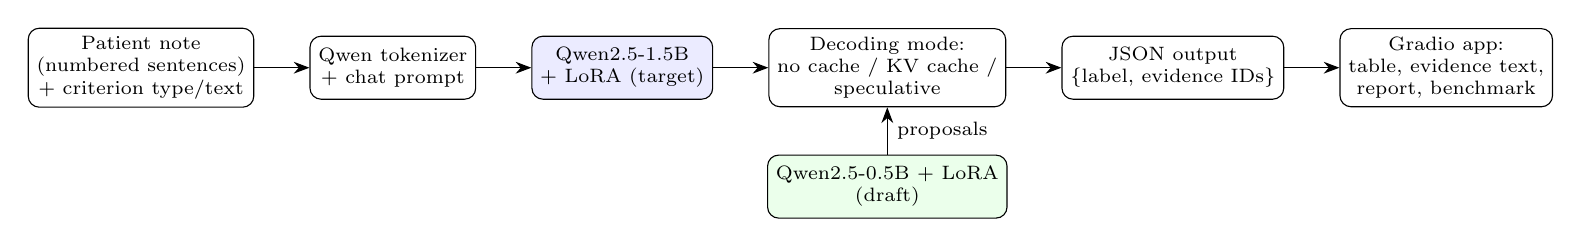
\begin{tikzpicture}[font=\scriptsize,node distance=7mm,box/.style={draw,rounded corners,align=center,minimum height=8mm,inner sep=3pt},arr/.style={-{Stealth[length=2mm]}}]
\node[box](in){Patient note\\(numbered sentences)\\+ criterion type/text};
\node[box,right=of in](tok){Qwen tokenizer\\+ chat prompt};
\node[box,right=of tok,fill=blue!8](tgt){Qwen2.5-1.5B\\+ LoRA (target)};
\node[box,right=of tgt](dec){Decoding mode:\\no cache / KV cache /\\speculative};
\node[box,right=of dec](out){JSON output\\\{label, evidence IDs\}};
\node[box,right=of out](app){Gradio app:\\table, evidence text,\\report, benchmark};
\node[box,below=6mm of dec,fill=green!8](drf){Qwen2.5-0.5B + LoRA\\(draft)};
\draw[arr](in)--(tok);\draw[arr](tok)--(tgt);\draw[arr](tgt)--(dec);\draw[arr](dec)--(out);\draw[arr](out)--(app);
\draw[arr](drf)--node[right]{proposals}(dec);
\end{tikzpicture}
\caption{System overview: prompt construction, the LoRA-tuned target, the three decoding paths (the draft is used only in speculative mode) and the application.}\label{fig:arch}\end{figure*}

A chat prompt contains the numbered note, the criterion type and text, the allowed labels for that type, and asks for JSON only: \texttt{\{"label": ..., "evidence": [ids]\}}. Inclusion labels are \emph{included, not included, not enough information, not applicable}; exclusion labels are \emph{excluded, not excluded, not enough information, not applicable}. Outputs are parsed strictly; unparsable or out-of-vocabulary outputs are counted as the label ``invalid'' (wrong), never silently repaired.
\subsection{LoRA fine-tuning}
The target is Qwen2.5-1.5B-Instruct \cite{qwen25}. LoRA adapters (rank 16, $\alpha{=}32$, dropout 0.05) are placed on all linear projections. Loss is computed on the answer tokens only. Settings: lr $2\times10^{-4}$ with cosine decay and 6 warm-up steps, 3 epochs, per-device batch 1 with 16 accumulation steps, fp16 autocast with fp32 adapter weights, gradient checkpointing, seed 42. The checkpoint with the lowest validation loss is kept (step 80). A second variant (v2) oversamples rare classes; it was trained for comparison and is reported below. A 0.5B draft adapter was trained with the same recipe for speculative decoding. Fig.~\ref{fig:curves} shows the training curves.
\begin{figure*}[t]\centering\safefig{train_curves}{0.95\textwidth}{}\caption{Training and validation loss (log scale); dotted line marks the selected checkpoint.}\label{fig:curves}\end{figure*}

\subsection{Metrics}
Overall and per criterion type: accuracy, macro-F1 (over classes present in the gold labels of that split), per-class precision/recall/F1 and confusion matrices. Evidence is scored on sentence-ID sets with micro P/R/F1 over all records and a per-record macro average in which an empty gold set matched by an empty prediction counts as correct. Because many records have empty gold evidence, we also report micro metrics restricted to non-empty gold.

\section{Results}
\subsection{Experimental setup}
All models are evaluated on identical validation and test records with greedy decoding (\texttt{do\_sample=False}), at most 64 new tokens, batch size 8, fp16; a full test pass takes about 27 s on the T4. The same prompt is used before and after fine-tuning, so the base model's low score also reflects format-following failures (parse failures count as wrong). Records with empty gold evidence are handled as described under Metrics.
\subsection{Before vs.\ after fine-tuning}
Table~\ref{tab:val} (validation) and Table~\ref{tab:test} (test, evaluated once after model selection) compare the base model with fine-tuned variants. The final model is v1 (plain LoRA), chosen on validation accuracy and validation loss before any test evaluation. The oversampled variant v2 has slightly higher validation macro-F1 and evidence F1 but lower accuracy; on test it again trades accuracy (0.714 vs 0.748) and exclusion macro-F1 for higher evidence precision. Given supports of 1--3 for rare classes these differences are within noise, and we did not switch models after seeing test results. Evidence results are in Table~\ref{tab:evid}; the high per-record macro F1 is inflated by records whose gold evidence is empty.
\begin{table*}[t]\centering\caption{Validation results.}\label{tab:val}\sm\safeinput{summary_val}\end{table*}
\begin{table*}[t]\centering\caption{Test results (single evaluation).}\label{tab:test}\sm\safeinput{summary_test}\end{table*}
\begin{table*}[t]\centering\caption{Evidence-sentence metrics, test split (see also the validation analogue in the repo).}\label{tab:evid}\sm\safeinput{evidence_test}\end{table*}

\subsection{Per-class behaviour}
Table~\ref{tab:pc} and Fig.~\ref{fig:cm} show per-class scores and confusion matrices on the test split for the final model. Majority classes (\emph{included}, \emph{not excluded}, inclusion \emph{not enough information}) are learned. The clearest failure is exclusion \emph{not enough information}: recall is 0.04 (28 gold cases, almost all predicted \emph{not excluded}), so the model treats missing information as absence of the exclusion condition. \emph{Not included} (7) and inclusion \emph{not applicable} (3) are never predicted correctly. The test split contains no \emph{excluded} case, so that class has no support there (validation had 2, also missed). Classes with a handful of examples are unreliable, since one example moves their F1 in large steps.
\begin{table}[t]\centering\caption{Per-class results, final model, test.}\label{tab:pc}\scriptsize\setlength{\tabcolsep}{3pt}\safeinput{perclass_test}\end{table}
\begin{figure*}[t]\centering\safefig{cm_test}{0.8\textwidth}{}\caption{Test confusion matrices (counts; colour is row-normalised).}\label{fig:cm}\end{figure*}

\subsection{Error analysis}
Table~\ref{tab:err} lists twelve test errors chosen automatically from distinct (gold, predicted) groups, at most two per group and patient. The recurring categories are: (i) a failed inclusion criterion not recognised, so \emph{not included} becomes \emph{not enough information} (rows 1--2); (ii) missing information treated as absence, so \emph{not enough information} becomes \emph{not excluded}; (iii) non-applicability not recognised, e.g.\ breast-feeding, birth-control or prior-tonsillectomy criteria answered as \emph{not excluded} or \emph{not enough information} (rows 3--6); (iv) correct label with wrong or missing cited sentences (rows 11--12), and over-caution, where an \emph{included} criterion is answered \emph{not enough information} (row 10). In several rows the model cites no sentence at all although the gold evidence is non-empty, which matches the low evidence recall (0.52). \todo{author: read errors.json and check these interpretations against the notes}
\begin{table*}[t]\centering\caption{Test errors of the final model (full text in \texttt{report/generated/errors.json}).}\label{tab:err}\scriptsize\safeinput{errors}\end{table*}

\section{KV-Cache Decoder}
\texttt{generate\_cached} runs an explicit prefill and then one token per step, passing explicit \texttt{position\_ids}, a growing attention mask and the carried cache; \texttt{generate\_nocache} recomputes the full sequence each step and is the reference. Table~\ref{tab:kv} compares them (greedy, batch 1, fixed number of new tokens, fp16, one warm-up run and the median of three timed runs with CUDA synchronisation). The speed-up grows with input length (1.1$\times$ at 128 tokens, 4.5$\times$ at 512 with 64 new tokens) because the reference cost grows with sequence length while a cached step does not; peak memory differs little at these lengths because weights dominate, and the KV cache itself is small (GQA with 2 KV heads). In one configuration (256 in / 64 new) the token streams diverge at step 20; an fp32 re-run was identical, so the divergence is an fp16 near-tie in the argmax, not a cache bug.
\begin{table*}[t]\centering\caption{KV cache vs.\ no-cache reference.}\label{tab:kv}\scriptsize\safeinput{kv}\end{table*}

\section{Tiled Attention}
\texttt{tiled\_attention} processes queries and keys in blocks keeping a running row maximum $m$, normaliser $\ell$ and accumulator $a$: for each key block with scores $S$, $m'=\max(m,\max S)$, $\ell\leftarrow \ell e^{m-m'}+\sum e^{S-m'}$, $a\leftarrow a e^{m-m'}+e^{S-m'}V$, and the output is $a/\ell$ \cite{milakov}. It never materialises the full $T_q\times T_k$ matrix, skips fully masked causal blocks, supports $T_q<T_k$ via an offset, and guards $-\infty-(-\infty)$. Table~\ref{tab:at} cross-checks it against a stable reference softmax and PyTorch SDPA (\safeinput{attn_tests_note}).
\begin{table}[t]\centering\caption{Tiled attention correctness (fp32).}\label{tab:at}\scriptsize\safeinput{attn_tests}\end{table}
Table~\ref{tab:ab} and Fig.~\ref{fig:ab} give timing and peak extra memory. Our tiled version is written in PyTorch loops, so it is not expected to beat the fused SDPA kernel in time; its value is the memory behaviour and the verified algorithm.
\begin{table}[t]\centering\caption{Attention timing / memory (batch 1, 12 heads, $D{=}128$).}\label{tab:ab}\scriptsize\safeinput{attn_bench}\end{table}
\begin{figure*}[t]\centering\safefig{attn_bench}{0.8\textwidth}{}\caption{Attention benchmark.}\label{fig:ab}\end{figure*}

\section{Speculative Decoding}
A 0.5B draft (same tokenizer, asserted in code) proposes $k$ tokens greedily; the 1.5B target verifies $[\text{last}]+\text{drafts}$ in one pass, the longest agreeing prefix is accepted, and the target's own next token is appended as correction or bonus token. Both caches are cropped to hold exactly the accepted sequence; the invariant at the start of a round is that both caches hold KV for all tokens but the last. Output is identical to the target's greedy output (8/8 prompts equal). Table~\ref{tab:sp} shows speculative decoding was \emph{slower} than cached greedy decoding (0.65--0.76$\times$): with a 1.5B target the draft is only 3$\times$ smaller, acceptance is 0.5--0.7, and each round pays draft and verification overhead plus cache cropping in Python, whereas a cached 1.5B step is already cheap. Larger target/draft ratios, higher acceptance or batched verification would be needed for a gain.
\begin{table*}[t]\centering\caption{Speculative vs.\ greedy cached decoding (48 new tokens, 8 prompts).}\label{tab:sp}\scriptsize\safeinput{spec}\end{table*}

\section{Application}
The Gradio application has three tabs. (1) \emph{Screening}: the user pastes a patient description (plain text or dataset-style numbered sentences) and enters inclusion and exclusion criteria, one per line; a dropdown selects the decoding mode (KV cache, no-cache reference, speculative with adjustable $k$). The result shows, per criterion, the predicted category, cited sentence IDs, the exact evidence text, the raw model output and the time taken, followed by a preliminary outcome computed by an explicit rule (not a ground-truth verdict), and a downloadable Markdown report with provenance (models, adapters, decoding mode, timestamp, sentence handling). (2) \emph{Inference benchmark}: runs the first criterion live through no-cache, KV-cache and speculative decoding and reports time, tokens/s, speed-up, peak GPU memory, token equality with the reference, acceptance rate and target passes. (3) \emph{Held-out test results}: loads the stored test metrics. Invalid inputs (empty or too short notes, over-long input) raise a clear message and the app stays usable. A prominent notice states that this is an educational prototype, not a clinical enrolment decision (Figs.~\ref{fig:shot1} and~\ref{fig:shot2}).
\textbf{Startup.} The app is launched locally with \texttt{python app/app.py} and opened at \texttt{http://127.0.0.1:7860}; it downloads the base models and the published adapters and uses the GPU if present, otherwise the CPU. No notebook is needed. Exact steps are in the repository README.
\begin{figure}[t]\centering\safepng{app_screening}{0.95\columnwidth}\caption{Screening tab with per-criterion results, evidence and report download.}\label{fig:shot1}\end{figure}
\begin{figure}[t]\centering\safepng{app_benchmark}{0.95\columnwidth}\caption{Inference benchmark tab comparing the three decoding paths live.}\label{fig:shot2}\end{figure}

\section{Limitations}
Only 53 patients; validation/test supports of 1--3 for rare classes make per-class scores noisy and differences between v1 and v2 within noise. Model selection used the validation split and test was evaluated once for the final model. Greedy fp16 decoding can differ across hardware on near-ties. The public app link exists only while the notebook session runs. No clinical validation was performed.

\section{Conclusion}
LoRA fine-tuning makes a 1.5B decoder usable for criterion-level eligibility labelling (test accuracy 0.107 $\rightarrow$ 0.748, macro-F1 0.141 $\rightarrow$ 0.550), but rare classes, exclusion criteria with missing information, and evidence selection remain hard. The KV cache gives up to 4.5$\times$ speed-up at 512 tokens, tiled attention matches the reference to float precision, and speculative decoding preserved outputs but did not speed things up here.

\appendices
\section{AI-Use Statement}
An AI assistant (Claude) was used for planning, writing and debugging code (training, evaluation, KV cache, tiled attention, speculative decoding, app), generating figure/table scripts and drafting this report. All experiments were run by the author on Kaggle; numbers come from the committed JSON files. \todo{author: describe what you verified yourself and any parts you rewrote}

\begin{thebibliography}{10}
\bibitem{trialgpt} Q.~Jin \emph{et al.}, ``Matching patients to clinical trials with large language models,'' \emph{Nature Communications}, vol.~15, 2024.
\bibitem{lora} E.~J. Hu \emph{et al.}, ``LoRA: Low-rank adaptation of large language models,'' in \emph{ICLR}, 2022.
\bibitem{flash} T.~Dao \emph{et al.}, ``FlashAttention: Fast and memory-efficient exact attention with IO-awareness,'' in \emph{NeurIPS}, 2022.
\bibitem{milakov} M.~Milakov and N.~Gimelshein, ``Online normalizer calculation for softmax,'' arXiv:1805.02867, 2018.
\bibitem{leviathan} Y.~Leviathan, M.~Kalman, and Y.~Matias, ``Fast inference from transformers via speculative decoding,'' in \emph{ICML}, 2023.
\bibitem{chen} C.~Chen \emph{et al.}, ``Accelerating large language model decoding with speculative sampling,'' arXiv:2302.01318, 2023.
\bibitem{qlora} T.~Dettmers \emph{et al.}, ``QLoRA: Efficient finetuning of quantized LLMs,'' in \emph{NeurIPS}, 2023.
\bibitem{rabe} M.~N. Rabe and C.~Staats, ``Self-attention does not need $O(n^2)$ memory,'' arXiv:2112.05682, 2021.
\bibitem{pope} R.~Pope \emph{et al.}, ``Efficiently scaling transformer inference,'' in \emph{MLSys}, 2023.
\bibitem{gqa} J.~Ainslie \emph{et al.}, ``GQA: Training generalized multi-query transformer models from multi-head checkpoints,'' in \emph{EMNLP}, 2023.
\bibitem{rope} J.~Su \emph{et al.}, ``RoFormer: Enhanced transformer with rotary position embedding,'' arXiv:2104.09864, 2021.
\bibitem{qwen25} A.~Yang \emph{et al.}, ``Qwen2.5 technical report,'' arXiv:2412.15115, 2024.
\end{thebibliography}
\end{document}
